\documentclass{article}\usepackage[]{graphicx}\usepackage[]{color}
%% maxwidth is the original width if it is less than linewidth
%% otherwise use linewidth (to make sure the graphics do not exceed the margin)
\makeatletter
\def\maxwidth{ %
  \ifdim\Gin@nat@width>\linewidth
    \linewidth
  \else
    \Gin@nat@width
  \fi
}
\makeatother

\definecolor{fgcolor}{rgb}{0.345, 0.345, 0.345}
\newcommand{\hlnum}[1]{\textcolor[rgb]{0.686,0.059,0.569}{#1}}%
\newcommand{\hlstr}[1]{\textcolor[rgb]{0.192,0.494,0.8}{#1}}%
\newcommand{\hlcom}[1]{\textcolor[rgb]{0.678,0.584,0.686}{\textit{#1}}}%
\newcommand{\hlopt}[1]{\textcolor[rgb]{0,0,0}{#1}}%
\newcommand{\hlstd}[1]{\textcolor[rgb]{0.345,0.345,0.345}{#1}}%
\newcommand{\hlkwa}[1]{\textcolor[rgb]{0.161,0.373,0.58}{\textbf{#1}}}%
\newcommand{\hlkwb}[1]{\textcolor[rgb]{0.69,0.353,0.396}{#1}}%
\newcommand{\hlkwc}[1]{\textcolor[rgb]{0.333,0.667,0.333}{#1}}%
\newcommand{\hlkwd}[1]{\textcolor[rgb]{0.737,0.353,0.396}{\textbf{#1}}}%
\let\hlipl\hlkwb

\usepackage{framed}
\makeatletter
\newenvironment{kframe}{%
 \def\at@end@of@kframe{}%
 \ifinner\ifhmode%
  \def\at@end@of@kframe{\end{minipage}}%
  \begin{minipage}{\columnwidth}%
 \fi\fi%
 \def\FrameCommand##1{\hskip\@totalleftmargin \hskip-\fboxsep
 \colorbox{shadecolor}{##1}\hskip-\fboxsep
     % There is no \\@totalrightmargin, so:
     \hskip-\linewidth \hskip-\@totalleftmargin \hskip\columnwidth}%
 \MakeFramed {\advance\hsize-\width
   \@totalleftmargin\z@ \linewidth\hsize
   \@setminipage}}%
 {\par\unskip\endMakeFramed%
 \at@end@of@kframe}
\makeatother

\definecolor{shadecolor}{rgb}{.97, .97, .97}
\definecolor{messagecolor}{rgb}{0, 0, 0}
\definecolor{warningcolor}{rgb}{1, 0, 1}
\definecolor{errorcolor}{rgb}{1, 0, 0}
\newenvironment{knitrout}{}{} % an empty environment to be redefined in TeX

\usepackage{alltt}
\usepackage{gensymb}

\title{Visual Presentation of Data using R}



\IfFileExists{upquote.sty}{\usepackage{upquote}}{}
\begin{document}
\maketitle

\section{The Perfect Graphic}

\subsection{Best Practices}

There is no such thing as the perfect graphic, but there are conventions that can be used to guide us to create accurtate, accessible, and visually pleasing grahics. But like many things, it takes some practices. 

Here are some general rules...

\begin{itemize}
  \item Data range and transformations
  \item Axes labels with appropriate units
  \item Axes label and values font size
  \item Axes label orientation
  \item Title
  \item lines and points
  \item B/W versus color
  \item Caption
\end{itemize}


\section{Exploring the Histogram}

Data exploration can include many steps, but starting with a histogram gives the researcher the ability to evaluate the distribution of the data.

Below is a default histogram for TMAX values, where we might be able to visually how normally distributed the data might be.

\begin{knitrout}
\definecolor{shadecolor}{rgb}{0.969, 0.969, 0.969}\color{fgcolor}\begin{kframe}
\begin{alltt}
\hlkwd{hist}\hlstd{(MonthlyTMAXMean}\hlopt{$}\hlstd{TMAX)}
\end{alltt}
\end{kframe}
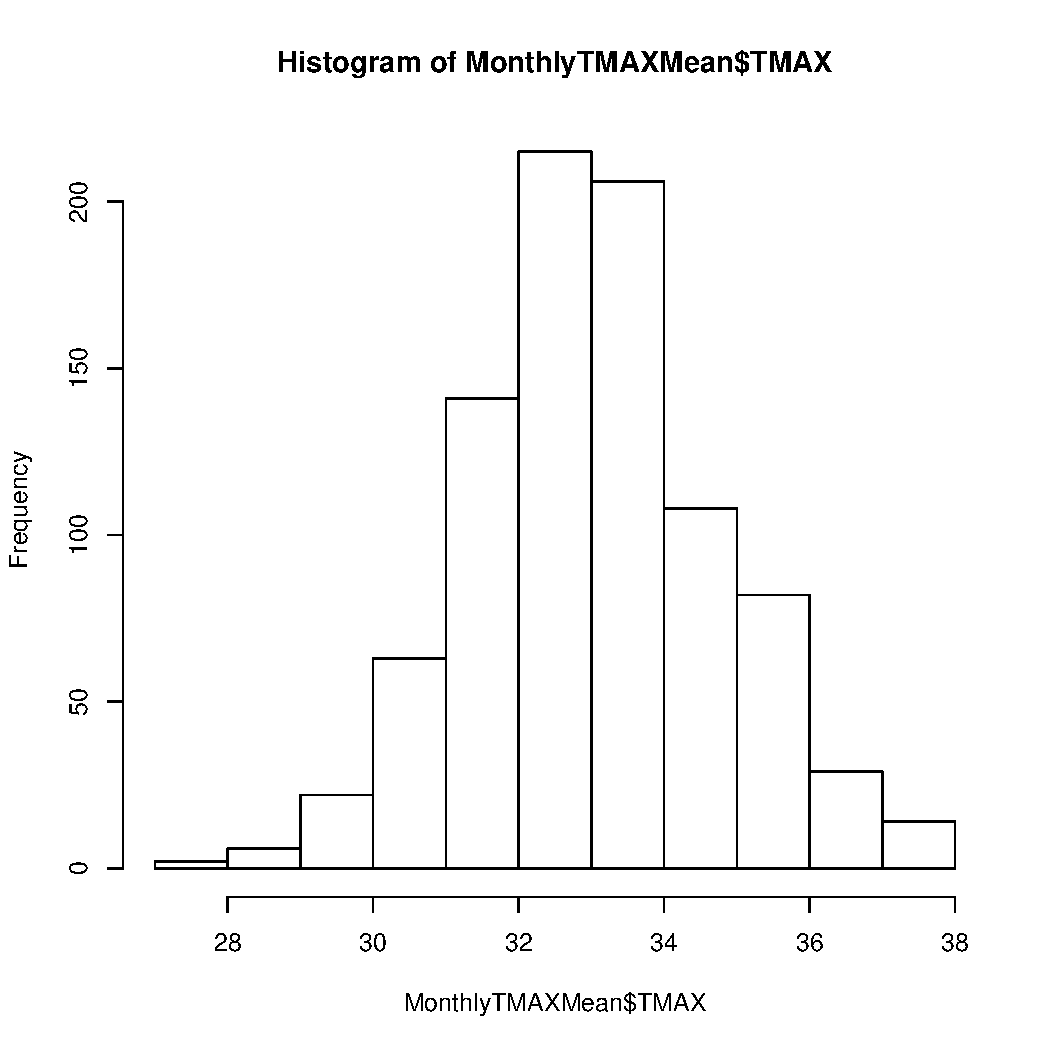
\includegraphics[width=\maxwidth]{figure/unnamed-chunk-2-1} 

\end{knitrout}

The default graphic is hideous -- so, let's start fixing it. 

\subsection{Title and Axis Labels}

For stand alone figures, we usually add titles, but in papers and lab reports it's a good practice to remove the title and use the caption to describe the graphic. Changes to the title can be made with arguments within the plot command, i.e. `main=NULL'.

In addition, we can change the x-axis label, with the 'xlab' argument. Specifying the units is also required. And in this case, we want to add the \degree symbol and create a text string with the axis label in quotes that can be referenced in the hist() funtion. 

\begin{knitrout}
\definecolor{shadecolor}{rgb}{0.969, 0.969, 0.969}\color{fgcolor}\begin{kframe}
\begin{alltt}
\hlstd{TMAXlabel} \hlkwb{<-} \hlstr{"Maximum Temperature (°C)"}
\hlkwd{hist}\hlstd{(MonthlyTMAXMean}\hlopt{$}\hlstd{TMAX,} \hlkwc{main}\hlstd{=}\hlkwa{NULL}\hlstd{,} \hlkwc{xlab}\hlstd{=TMAXlabel)}
\end{alltt}
\end{kframe}
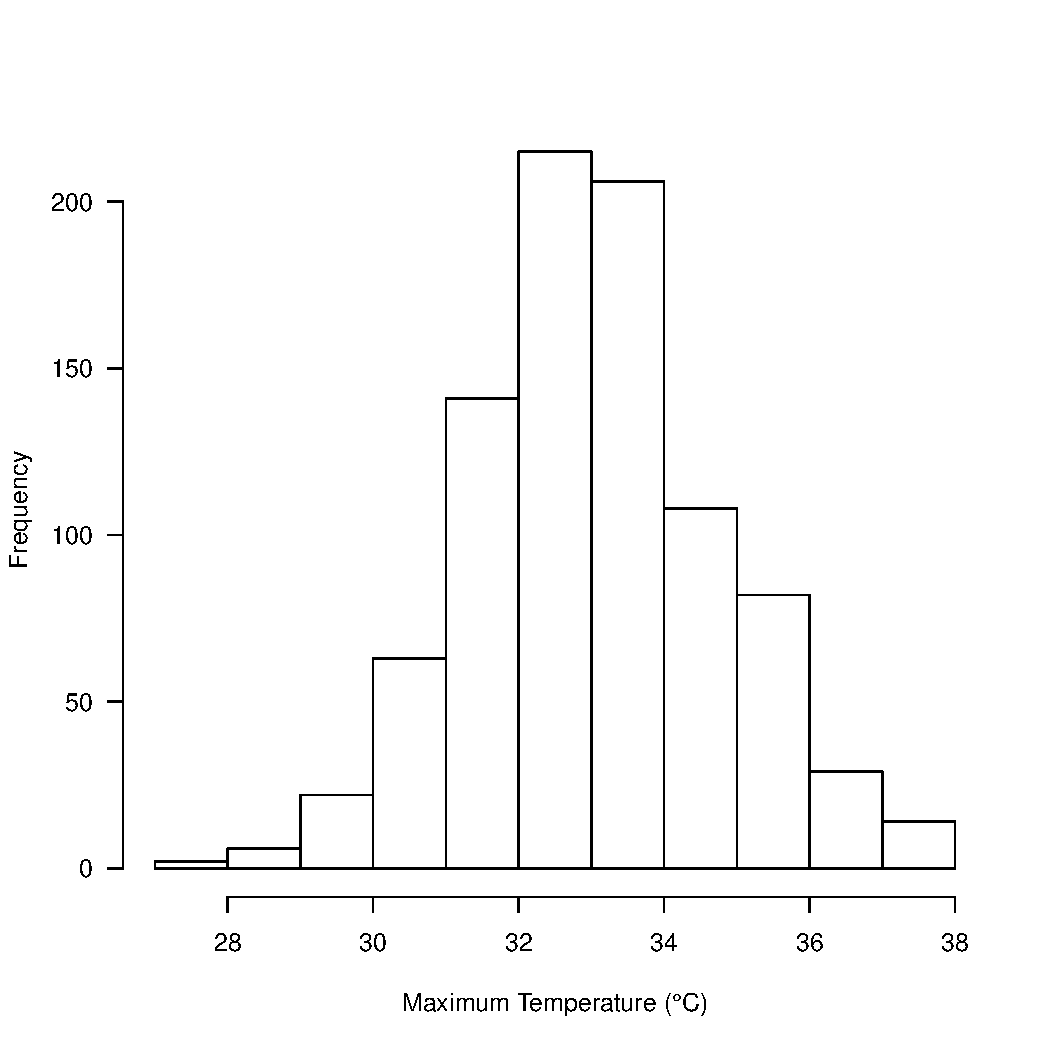
\includegraphics[width=\maxwidth]{figure/unnamed-chunk-3-1} 

\end{knitrout}

\subsection{Putting Multiple Figures in a Row}

To create two graphics in one row, we can change the graphic parameters with the par() function. In this case, we'll create two column panels in one row using the 'mfrow' option and a vector that defines the number of rows and the number of columns. It's often a good idea to set the graphic parameter back to the default afterwards. 

\begin{knitrout}
\definecolor{shadecolor}{rgb}{0.969, 0.969, 0.969}\color{fgcolor}\begin{kframe}
\begin{alltt}
\hlkwd{par}\hlstd{(}\hlkwc{mfrow}\hlstd{=}\hlkwd{c}\hlstd{(}\hlnum{1}\hlstd{,}\hlnum{2}\hlstd{))}
\hlkwd{hist}\hlstd{(MonthlyTMAXMean}\hlopt{$}\hlstd{TMAX,} \hlkwc{main}\hlstd{=}\hlkwa{NULL}\hlstd{,} \hlkwc{xlab}\hlstd{=TMAXlabel)}
\hlstd{TMINlabel} \hlkwb{<-} \hlstr{"Minimum Temperature (°C)"}
\hlkwd{hist}\hlstd{(MonthlyTMINMean}\hlopt{$}\hlstd{TMIN,} \hlkwc{main}\hlstd{=}\hlkwa{NULL}\hlstd{,} \hlkwc{xlab}\hlstd{=TMINlabel)}
\end{alltt}
\end{kframe}
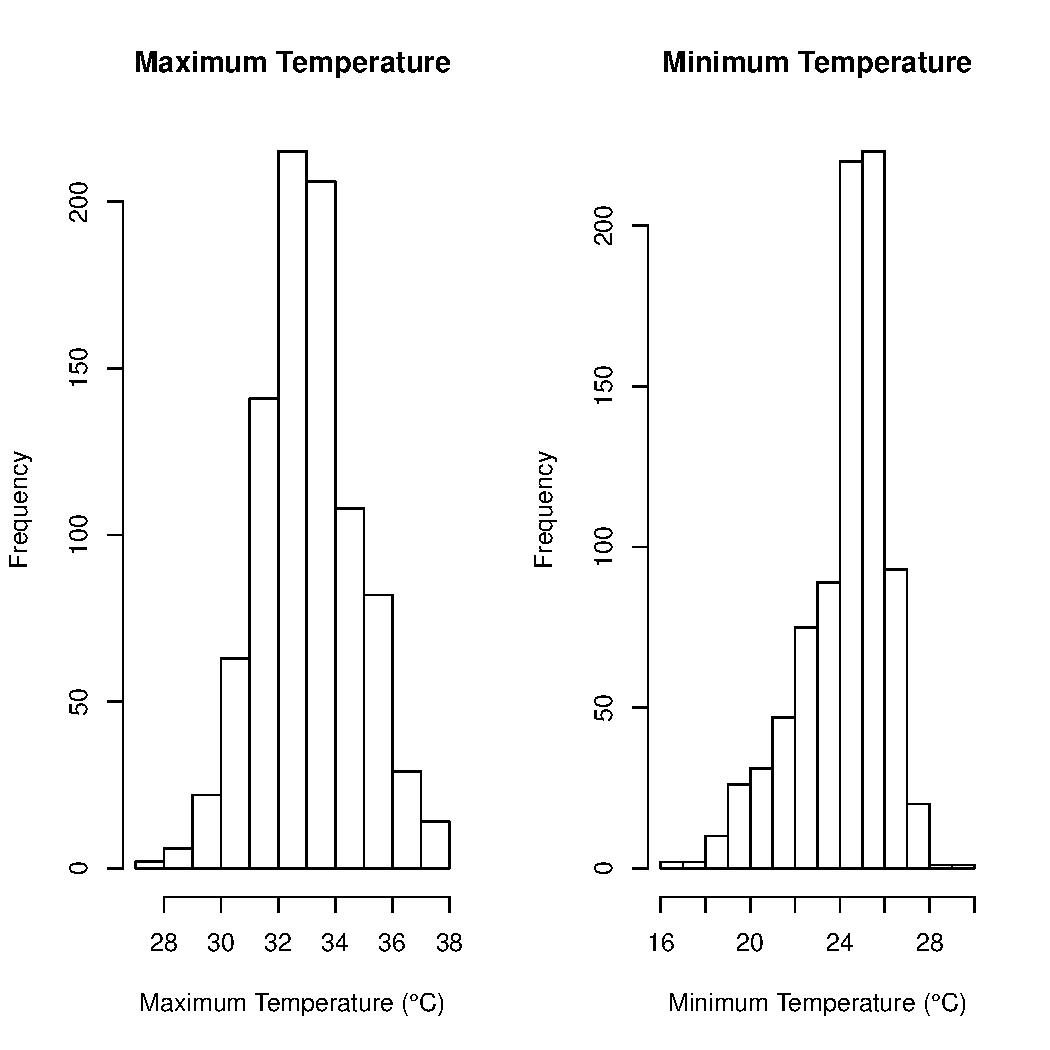
\includegraphics[width=\maxwidth]{figure/unnamed-chunk-4-1} 
\begin{kframe}\begin{alltt}
\hlkwd{par}\hlstd{(}\hlkwc{mfrow}\hlstd{=}\hlkwd{c}\hlstd{(}\hlnum{1}\hlstd{,}\hlnum{1}\hlstd{))}
\end{alltt}
\end{kframe}
\end{knitrout}


\section{Boxplot}



\section{Scatter Plot -- Non-time series}


\subsection{Scatter Plot -- Time Series}

For scatter plots, which are more common, we use the same principles:

\begin{knitrout}
\definecolor{shadecolor}{rgb}{0.969, 0.969, 0.969}\color{fgcolor}\begin{kframe}
\begin{alltt}
\hlkwd{plot}\hlstd{(TMAX} \hlopt{~} \hlstd{YEAR,} \hlkwc{data}\hlstd{=MonthlyTMAXMean[MonthlyTMAXMean}\hlopt{$}\hlstd{MONTH}\hlopt{==}\hlnum{5}\hlstd{,])}
\hlkwd{abline}\hlstd{(}\hlkwd{coef}\hlstd{(}\hlkwd{lm}\hlstd{(TMAX} \hlopt{~} \hlstd{YEAR,} \hlkwc{data}\hlstd{=MonthlyTMAXMean[MonthlyTMAXMean}\hlopt{$}\hlstd{MONTH}\hlopt{==}\hlnum{5}\hlstd{,])),}
    \hlkwc{col}\hlstd{=}\hlstr{'darkred'}\hlstd{)}
\end{alltt}
\end{kframe}
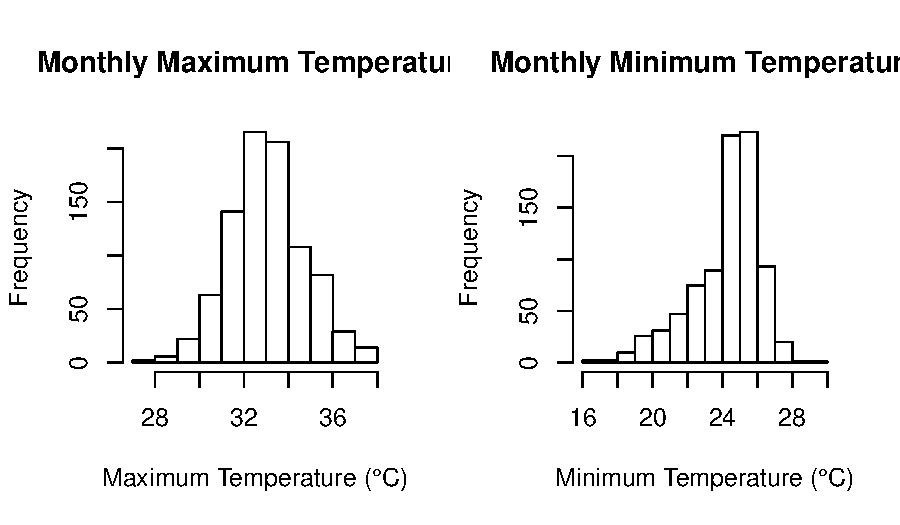
\includegraphics[width=\maxwidth]{figure/unnamed-chunk-5-1} 

\end{knitrout}

Let's fix the y-axis label as we did above (TMAX is not a very helpful label!). Furthermore, the x-axis needs to be calmed down some, so let's change the case for these. We will also change the symbols to make it less busy with the `pch' argument. You can look online to see the choices one has in R. 

I am also not impress with the vertical orientation of the y-axis, so it's important to change these as well. 

Finally, it's important that the image works in black and white. So, let's see if we can modify the graphic to make it less resource intensive. Finally, let's add a caption and reference to the figure (Figure \ref{fig:maxtemp}).

\begin{figure}[h]
\begin{knitrout}
\definecolor{shadecolor}{rgb}{0.969, 0.969, 0.969}\color{fgcolor}\begin{kframe}
\begin{alltt}
\hlstd{ylabel} \hlkwb{<-} \hlstr{"Maximum Temperature (°C)"}
\hlkwd{plot}\hlstd{(TMAX} \hlopt{~} \hlstd{YEAR,} \hlkwc{data}\hlstd{=MonthlyTMAXMean[MonthlyTMAXMean}\hlopt{$}\hlstd{MONTH}\hlopt{==}\hlnum{5}\hlstd{,],}
     \hlkwc{ylab}\hlstd{=ylabel,} \hlkwc{xlab}\hlstd{=}\hlstr{'Year'}\hlstd{,} \hlkwc{pch}\hlstd{=}\hlnum{20}\hlstd{,} \hlkwc{las}\hlstd{=}\hlnum{1}\hlstd{,} \hlkwc{col}\hlstd{=}\hlstr{'gray'}\hlstd{)}

\hlkwd{abline}\hlstd{(}\hlkwd{coef}\hlstd{(}\hlkwd{lm}\hlstd{(TMAX} \hlopt{~} \hlstd{YEAR,}
    \hlkwc{data}\hlstd{=MonthlyTMAXMean[MonthlyTMAXMean}\hlopt{$}\hlstd{MONTH}\hlopt{==}\hlnum{5}\hlstd{,])),} \hlkwc{col}\hlstd{=}\hlstr{'black'}\hlstd{)}
\end{alltt}
\end{kframe}
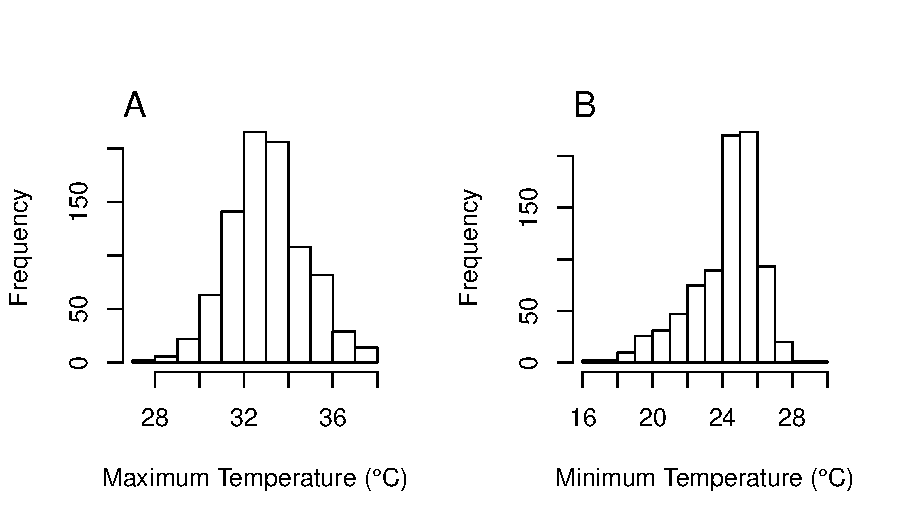
\includegraphics[width=\maxwidth]{figure/unnamed-chunk-6-1} 

\end{knitrout}
\caption{Monthly Average of Daily Maximum Temperatures (\degree C).}
\label{fig:maxtemp}
\end{figure}

Now, what if we only want to display part of the data. We can limit the x-axis range using the 'xlim' argument, where we create a vector of for the start and end of the range.  

\begin{figure}[h]
\begin{knitrout}
\definecolor{shadecolor}{rgb}{0.969, 0.969, 0.969}\color{fgcolor}\begin{kframe}
\begin{alltt}
\hlstd{ylabel} \hlkwb{<-} \hlstr{"Maximum Temperature (°C)"}
\hlkwd{plot}\hlstd{(TMAX} \hlopt{~} \hlstd{YEAR,} \hlkwc{data}\hlstd{=MonthlyTMAXMean[MonthlyTMAXMean}\hlopt{$}\hlstd{MONTH}\hlopt{==}\hlnum{5}\hlstd{,],}
     \hlkwc{xlim}\hlstd{=}\hlkwd{c}\hlstd{(}\hlnum{1940}\hlstd{,} \hlnum{2000}\hlstd{),}
     \hlkwc{ylab}\hlstd{=ylabel,} \hlkwc{xlab}\hlstd{=}\hlstr{'Year'}\hlstd{,} \hlkwc{pch}\hlstd{=}\hlnum{20}\hlstd{,} \hlkwc{las}\hlstd{=}\hlnum{1}\hlstd{,} \hlkwc{col}\hlstd{=}\hlstr{'gray'}\hlstd{)}

\hlkwd{abline}\hlstd{(}\hlkwd{coef}\hlstd{(}\hlkwd{lm}\hlstd{(TMAX} \hlopt{~} \hlstd{YEAR,}
    \hlkwc{data}\hlstd{=MonthlyTMAXMean[MonthlyTMAXMean}\hlopt{$}\hlstd{MONTH}\hlopt{==}\hlnum{5}\hlstd{,])),} \hlkwc{col}\hlstd{=}\hlstr{'black'}\hlstd{)}
\end{alltt}
\end{kframe}
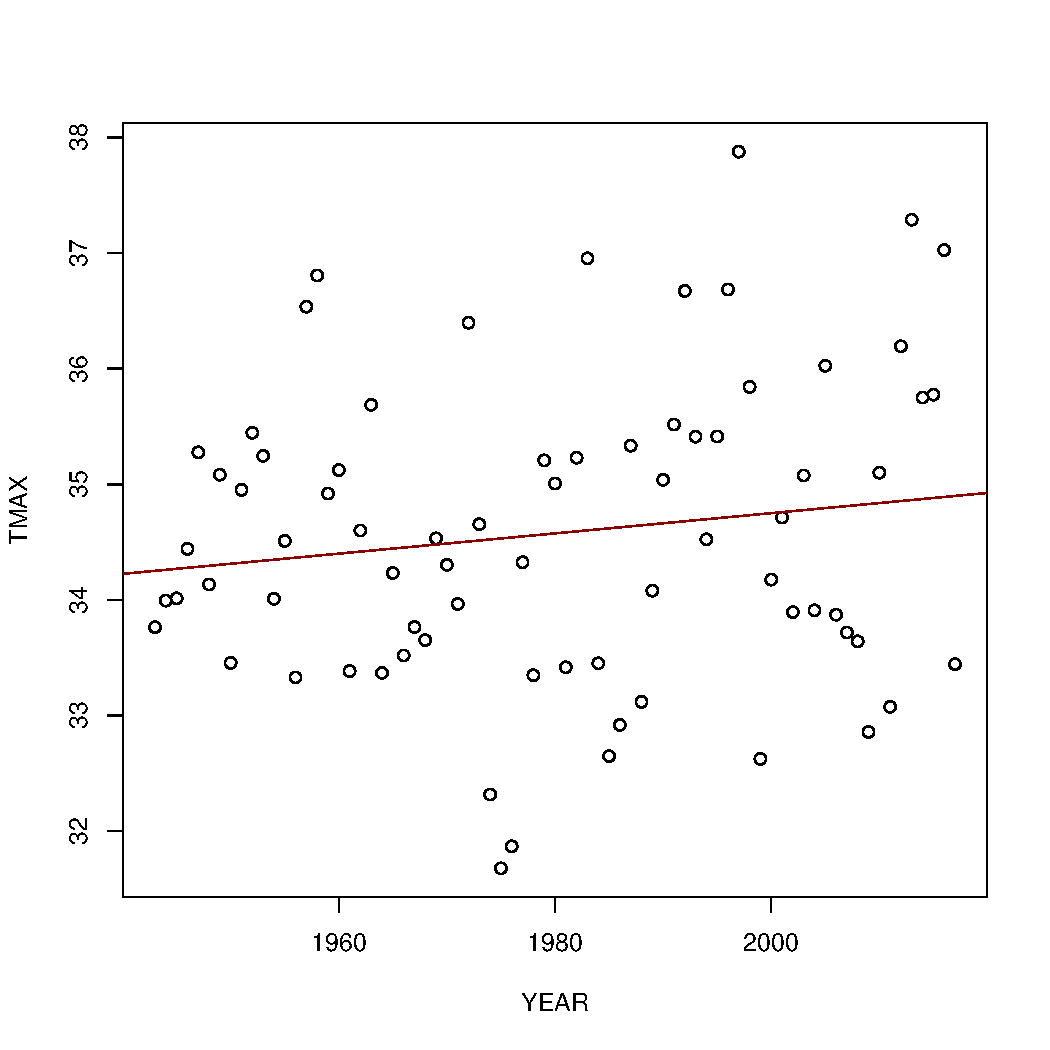
\includegraphics[width=\maxwidth]{figure/unnamed-chunk-7-1} 

\end{knitrout}
\caption{Monthly Average of Daily Maximum Temperatures (\degree C).}
\label{fig:maxtemp}
\end{figure}

Alternatively, you may want to creat a best fit line that only covers the range for the existing data without extrapolating, which is usually a very good idea for most scientific endeavors!




\section{Bar Graphs}


\section{Tables}



\end{document}
